\documentclass[10pt]{article}

\usepackage{amssymb,amsmath,amsthm}
\usepackage{bm}
\usepackage{graphicx,subcaption}
\usepackage[letterpaper, top=1in, left=1in, right=1in, bottom=1in]{geometry}
\usepackage{siunitx}

\newtheorem{definition}{Definition}
\newtheorem{theorem}{Theorem}
\newtheorem{lemma}{Lemma}
\newtheorem{remark}{Remark}

\newcommand{\SO}{\ensuremath{\mathrm{SO}(3)}}
\newcommand{\tr}[1]{\ensuremath{\mathrm{tr}\left( #1 \right)}}
\newcommand{\abs}[1]{\ensuremath{\left| #1 \right|}}
\newcommand{\diff}[1]{\mathrm{d}#1}
\newcommand{\vect}[1]{\ensuremath{\mathrm{vec}\left[ #1 \right]}}

\newcommand{\liediff}{\mathfrak{d}}
\newcommand{\dft}{\mathcal{F}}
\newcommand{\real}{\ensuremath{\mathbb{R}}}
\newcommand{\sph}{\ensuremath{\mathbb{S}}}
\newcommand{\diag}{\ensuremath{\mathrm{diag}}}

\title{\vspace{-4ex}\textbf{Uncertainty Propagation for a 3D Pendulum\vspace{-4ex}}}
\date{}

\begin{document}

\maketitle

The dynamical model for a hinged 3D pendulum is
\begin{align*}
	R^T\diff{R} &= \hat{\Omega}\diff{t} \\
	J\diff{\Omega} &= \left( -\Omega\times J\Omega - mg\rho\times R^Te_3 \right) \diff{t} + H\diff{W}_t,
\end{align*}
where $J\in\real^{3\times 3}$ is the moment of inertia matrix, $\rho$ is the vector from the pivot point to the center of mass expressed in the body-fixed frame.
The Fokker-Planck equation is
\begin{align} \label{eqn:FP}
	\frac{\partial p(R,\Omega,t)}{\partial t} = -\sum_{i=1}^{3} \liediff_i (\Omega_ip(R,\Omega,t)) + \sum_{i=1}^{3} \frac{\partial}{\partial \Omega_i} \left[(\Omega\times J\Omega + mg\rho\times R^Te_3)_i p(R,\Omega,t)\right] + \sum_{i,j=1}^{3} G_{ij} \frac{\partial^2 p(R,\Omega,t)}{\partial \Omega_i \partial \Omega_j}.
\end{align}
Let $F^l_{m,n,i,j,k}[p]$ be the Fourier coefficient of the probability density, then it satisfies the following ordinary different equation
\begin{align} \label{eqn:FP Fourier}
	\frac{\diff{F^l_{m,n,i,j,k}[p]}}{\diff{t}} = &-\sum_{\alpha=1}^3 F^l_{m,n,i,j,k}[\liediff_\alpha (\Omega_\alpha p)] + \sum_{\alpha=1}^3 F^l_{m,n,i,j,k}\left[ \frac{\partial}{\partial \Omega_\alpha}[(\Omega\times J\Omega + mg\rho\times R^Te_3)_\alpha p] \right] \nonumber \\
	&+ \sum_{\alpha,\beta=1}^3 G_{\alpha\beta} F^l_{m,n,i,j,k}\left[ \frac{\partial^2 p}{\partial\Omega_\alpha \partial\Omega_\beta} \right].
\end{align}

\section{Shape and Moment of Inertia}

Suppose the pendulum is a cylinder tube (Figure \ref{fig:pendulum}).
It is made of three materials: steel (red), aluminum (yellow), and acrylic (blue), and their densities are $\rho_1 = \SI{8050}{\kilogram\per\meter^3}$, $\rho_2 = \SI{2710}{\kilogram\per\meter^3}$, and $\rho_3 = \SI{1180}{\kilogram\per\meter^3}$ respectively.
The mass of the pendulum is
\begin{align}
	m = 0.5\pi(r_1^2-r_2^2)h_1(\rho_1+\rho_2) + \pi(r_1^2-r_2^2)h_2\rho_3 = \SI{1.85480}{\kilogram}.
\end{align}
The center of mass in the body-fixed frame is $\rho = \begin{bmatrix} 0 & 0 & \rho_z \end{bmatrix}^T$ where $\rho_z$ is
\begin{align}
	\rho_z = \frac{0.5(\rho_1+\rho_2)h_1 \cdot 0.5h_1 + \rho_3h_2(h_1+0.5h_2)}{0.5(\rho_1+\rho_2)h_1 + \rho_3h_2} = \SI{0.0679878}{\meter}.
\end{align}
The moment of inertial along body-fixed $e_1$-axis is
\begin{align}
	J_{11} &= 2\int_0^{h_1}\int_{r_2}^{r_1}\int_{\frac{\pi}{4}}^{\frac{3\pi}{4}} (r^2\sin^2\theta + z^2) r\rho_1 \diff{\theta} \diff{r} \diff{z} + 2\int_0^{h_1}\int_{r_2}^{r_1}\int_{-\frac{\pi}{4}}^{\frac{\pi}{4}} (r^2\sin^2\theta + z^2) r\rho_2 \diff{\theta} \diff{r} \diff{z} \nonumber \\
	&\qquad\qquad + \int_{h_1}^{h_1+h_2} \int_{r_1}^{r_2} \int_0^{2\pi} (r^2\sin^2\theta + z^2) r\rho_2 \diff{\theta} \diff{r} \diff{z} \nonumber \\
	&= \left( \frac{\pi+2}{8}\rho_1 + \frac{\pi-2}{8}\rho_2 \right)h_1(r_1^4-r_2^4) + \frac{\pi}{6} h_1^3(r_1^2-r_2^r)(\rho_1+\rho_2) + \frac{\pi}{4}(r_1^4-r_2^4)h_2\rho_3 \nonumber \\
	&\qquad\qquad + \frac{\pi}{3}(r_1^2-r_2^2)((h_1+h_2)^3-h_1^3)\rho_3 = \SI{0.0152492}{\kilogram\cdot\meter^2},
\end{align}
Similarly, the moment of inertial along body-fixed $e_2$-axis is
\begin{align}
	J_{22} &= \left( \frac{\pi-2}{8}\rho_1 + \frac{\pi+2}{8}\rho_2 \right)h_1(r_1^4-r_2^4) + \frac{\pi}{6} h_1^3(r_1^2-r_2^r)(\rho_1+\rho_2) + \frac{\pi}{4}(r_1^4-r_2^4)h_2\rho_3 \nonumber \\
	&\qquad\qquad + \frac{\pi}{3}(r_1^2-r_2^2)((h_1+h_2)^3-h_1^3)\rho_3 = \SI{0.0142639}{\kilogram\cdot\meter^2}.
\end{align}
The moment of inertial along body-fixed $e_3$-axis is
\begin{align}
	J_{33} &= \int_0^{h_1} \int_{r_1}^{r_2} \int_0^{\pi} r^3(\rho_1+\rho_2) \diff{\theta} \diff{r} \diff{z} + \int_{h_1}^{h_1+h_2} \int_{r_1}^{r_2} \int_0^\pi r^3\rho_3 \diff{\theta} \diff{r} \diff{z} \nonumber \\
	&= \frac{\pi}{4}(r_1^4-r_2^4)h_1(\rho_1+\rho_2) + \frac{\pi}{2}(r_1^4-r_2^4)h_2\rho_3 = \SI{0.00380233}{\kilogram\cdot\meter^2}
\end{align}

\begin{figure}
	\centering
	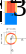
\includegraphics{pendulum.png}
	\caption{Dimensions of the pendulum \label{fig:pendulum}}
\end{figure}

\subsection{Scale Gravity}

Let $t = \alpha\tilde{t}$, and $\Omega = \tfrac{1}{\alpha}\tilde{\Omega}$, then the equation of motion can be rewritten as
\begin{align*}
	R^T\diff{R} &= \hat{\tilde{\Omega}} \diff{\tilde{t}} \\
	J\diff{\tilde{\Omega}} &= (-\tilde{\Omega}\times J\tilde{\Omega} - \alpha^2mg\rho\times R^Te_3) \diff{\tilde{t}} + \alpha^{3/2} H \diff{W_{\tilde{t}}}.
\end{align*}
Using the above equations, we can define $\tilde{g} = \alpha^2 g$ as an arbitrary number.
Let $\alpha^2 = \frac{J_{11}}{mg\rho_z}$, $\tilde{J} = \frac{1}{J_{11}}J$, and $\tilde{H} = \alpha^{3/2}J^{-1}H$, then the above equations can be further simplified as
\begin{align*}
	R^T\diff{R} &= \hat{\tilde{\Omega}} \diff{\tilde{t}} \\
	\diff{\tilde{\Omega}} &= \tilde{J}^{-1} (-\tilde{\Omega}\times \tilde{J}\tilde{\Omega} - e_3\times R^Te_3) \diff{\tilde{t}} + \tilde{H}\diff{W_{\tilde{t}}}.
\end{align*}

\section{Elastic Collision}
Suppose there is a wall perpendicular to $e_1$-axis, which intersects $e_1$-axis at $b$.
Then the collision criterion is given by $\theta \geq \theta_0$, where $\theta$ is the angle between the body-fixed $e_3$ axis and the inertial $e_2$-$e_3$ plane.
More specifically, $\theta$ is given by
\begin{align}
	\theta = 90^\circ - \arccos(t_3 \cdot e_1),
\end{align}
where $t_3$ is the third column of $R$.
Also, $\theta_0$ is a fixed value given by
\begin{align}
	\theta_0 = \arcsin\left(\frac{b}{\sqrt{h^2+r_1^2}}\right) - \arcsin\left(\frac{r_1}{\sqrt{h^2+r_1^2}}\right).
\end{align}
Suppose before collision, the angular velocity is given by $\Omega^-$.
The collision point in the inertial frame is given by
\begin{align}
	\rho_c = r_1 (\sec\theta\cdot e_1 - \tan\theta \cdot t_3).
\end{align}
Thus, the linear velocity at the collision point before collision in the inertial frame is
\begin{align}
	v_c^- = R\Omega^- \times \rho_c.
\end{align}
The velocity $v_c^-$ can be decomposed into the component along $e_1$, and perpendicular to $e_1$:
\begin{align}
	v_c^- &= (R\Omega^-\times\rho_c \cdot e_1)e_1 + v_c^- - (R\Omega^-\times\rho_c \cdot e_1)e_1 \nonumber \\
	&= -\left(r_1\tan\theta R(\Omega^-\times e_3)\cdot e_1\right)e_1 + v_c^- + \left(r_1\tan\theta R(\Omega^-\times e_3)\cdot e_1\right)e_1.
\end{align}
So the velocity at the collision point after collision in the inertial frame becomes
\begin{align}
	v_c^+ = v_c^- + 2(r_1\tan\theta R(\Omega^-\times e_3)\cdot e_1) e_1.
\end{align}
And the angular velocity after collision becomes the solution to
\begin{align}
	R\Omega^+ \times \rho_c = v_c^+.
\end{align}

\section{Marginal Density}

\begin{lemma} \label{lemma:marginal Fourier}
	Let $f(R,x)\in\mathcal{L}^2(\SO\times\real^N)$, and $F^l_{m,n,\mathcal{J}}$ be its Fourier coefficients, where $\mathcal{J} = \{j_1,\ldots,j_N\} \in \mathcal{N}^N$.
	Also, let $\tilde{f}(x) = \int_{R\in\SO} f(R,x) \diff{R}$, and $\tilde{F}_\mathcal{J}$ be its Fourier coefficients.
	Then
	\begin{align} \label{eqn:F_J}
		\tilde{F}_{\mathcal{J}} = F^0_{0,0,\mathcal{J}}.
	\end{align}
\end{lemma}
\begin{proof}
	First, $f(R,x)$ can be expanded as
	\begin{align*}
		f(R,x) = \sum_{l=0}^\infty \sum_{m,n=-l}^l \sum_{j'_1,\ldots,j'_N=-\infty}^\infty (2l+1) F^l_{m,n,\mathcal{J}'} D^l_{m,n}(R) \exp\left( \frac{2\pi i}{L} \sum_{\alpha=1}^N j'_\alpha x_\alpha \right).
	\end{align*}
	So we have
	\begin{align} \label{eqn:F_J calculation}
		\tilde{F}_\mathcal{J} &= \frac{1}{L^N} \int_{x\in[-L/2,L/2]^N} \int_{R\in\SO} f(R,x) \diff{R} \exp\left( -\frac{2\pi i}{L} \sum_{\alpha=1}^N j_\alpha x_\alpha \right) \diff{x} \nonumber \\
		&= \frac{1}{L^N} \sum_{j'_1,\ldots,j'_N=-\infty}^\infty \bigg[ \int_{x\in[-L/2,L/2]^N}  \exp\left( \frac{2\pi i}{L} \sum_{\alpha=1}^N j'_\alpha x_\alpha \right) \exp\left( -\frac{2\pi i}{L} \sum_{\alpha=1}^N j_\alpha x_\alpha \right) \diff{x} \nonumber \\
		&\qquad\qquad \times \int_{R\in\SO} \sum_{l=0}^{\infty} \sum_{m,n=-l}^l (2l+1)F^l_{m,n,\mathcal{J}'} D^l_{m,n}(R) \diff{R} \bigg] \nonumber \\
		&= \sum_{j'_1,\ldots,j'_N=-\infty}^\infty \delta_\mathcal{J}^{\mathcal{J}'} \sum_{l=0}^\infty \sum_{m,n=-l}^l (2l+1)F^l_{m,n,\mathcal{J}'} \int_{R\in\SO} D^l_{m,n}(R) \diff{R}.
	\end{align}
	Next, the integral of $D^l_{m,n}(R)$ can be directly calculated as
	\begin{align*}
		\int_{R\in\SO} D^l_{m,n}(R) \diff{R} &= \frac{1}{8\pi^2} \int_0^{2\pi} \int_0^\pi \int_0^{2\pi} e^{-im\alpha} d^l_{m,n}(\beta) e^{-in\gamma} \sin\beta \diff{\alpha} \diff{\beta} \diff{\gamma} \\
		&= \frac{1}{2} \delta_m^0 \delta_n^0 \int_0^\pi d^l_{0,0}(\beta) \sin\beta \diff{\beta} = \frac{1}{2} \delta_m^0 \delta_n^0 \int_0^\pi P_l(\cos\beta) \sin\beta \diff{\beta} = \delta_m^0 \delta_n^0 \delta_l^0.
	\end{align*}
	Thus, \eqref{eqn:F_J calculation} reduces to \eqref{eqn:F_J}.
\end{proof}

Let $p(\Omega,t) = \int_{R\in\SO}p(R,\Omega,t)\diff{R}$ be the marginal density of $\Omega$, and denote $F_{i,j,k}[p](t)$ as its Fourier coefficient.
Then using Lemma \ref{lemma:marginal Fourier}, $F_{i,j,k}[p](t)$ satisfied the ordinary differential equation
\begin{align} \label{eqn:FP marginal Fourier}
	\frac{\diff{F_{i,j,k}[p]}}{\diff{t}} =  \frac{\diff{F^0_{0,0,i,j,k}[p]}}{\diff{t}}.
\end{align}
Now let us calculate $\frac{\diff{F_{i,j,k}[p]}}{\diff{t}}$ by substituting \eqref{eqn:FP Fourier} into \eqref{eqn:FP marginal Fourier}.
First, the first term on the right hand side of \eqref{eqn:FP Fourier} is
\begin{align} \label{eqn:dF marginal}
	\frac{\diff{F^0_{0,0,i,j,k}[p]}}{\diff{t}} &= -\sum_{\alpha=1}^3 F^0_{0,0,i,j,k}[\liediff_\alpha(\Omega_\alpha p)] + \sum_{\alpha=1}^3 F^0_{0,0,i,j,k}\left[ \frac{\partial}{\partial \Omega_\alpha}[(\Omega\times J\Omega + mg\rho\times R^Te_3)_\alpha p] \right] \nonumber \\
	&\qquad\qquad +\sum_{\alpha,\beta=1}^3 G_{\alpha\beta} F^0_{0,0,i,j,k}\left[ \frac{\partial^2 p}{\partial\Omega_\alpha \partial\Omega_\beta} \right] \nonumber \\
	&= -\sum_{\alpha=1}^3 F_{i,j,k} \left[ \int_{R\in\SO} \liediff_\alpha(\Omega_\alpha p(R,\Omega,t)) \diff{R} \right] + \sum_{\alpha=1}^3 F_{i,j,k} \left[ \int_{R\in\SO} \frac{\partial}{\partial \Omega_\alpha}[(\Omega\times J\Omega)_\alpha p(R,\Omega,t)] \diff{R} \right] \nonumber \\
	&\qquad\qquad + \sum_{\alpha=1}^3 F^0_{0,0,i,j,k}\left[ \frac{\partial}{\partial \Omega_\alpha}[(mg\rho\times R^Te_3)_\alpha p] \right] + \sum_{\alpha,\beta=1}^3 G_{\alpha\beta} F_{i,j,k} \left[ \int_{R\in\SO} \frac{\partial^2 p(R,\Omega,t)}{\partial\Omega_\alpha \partial \Omega_\beta} \diff{R} \right] \nonumber \\
	&= -\sum_{\alpha=1}^3 F_{i,j,k} \left[ \frac{\partial}{\partial \Omega_\alpha} [(\Omega\times J\Omega)_\alpha p(\Omega,t)] \right] + \sum_{\alpha=1}^3 F^0_{0,0,i,j,k}\left[ \frac{\partial}{\partial \Omega_\alpha}[(mg\rho\times R^Te_3)_\alpha p(R,\Omega,t)] \right] \nonumber \\
	&\qquad\qquad + \sum_{\alpha,\beta=1}^3 G_{\alpha\beta} F_{i,j,k} \left[ \frac{\partial^2 p(\Omega,t)}{\partial \Omega_\alpha \partial \Omega_\beta} \right].
\end{align}
where the last equality comes the from the following lemma
\begin{lemma} \label{lemma:integrating derivative}
	Let $f\in C^1(\SO)$, then $\int_{R\in\SO} \liediff_i f \diff{R} = 0$ for $i=1,2,3$.
\end{lemma}
\begin{proof}
	It can be directly calculated as:
	\begin{align*}
		\int_{R\in\SO} \liediff_i f\diff{R} &= \int_{R\in\SO} \frac{\diff{}}{\diff{t}} \bigg\lvert_{t=0} f(R\exp(t\hat{e}_i)) \diff{R} \\
		&= \lim\limits_{t\to 0} \frac{1}{t} \left( \int_{R\in\SO} f(R\exp(t\hat{e}_i)) \diff{R} - \int_{R\in\SO} f(R) \diff{R} \right) = 0.
	\end{align*}
	Note that the last equality is because the term in the big parentheses is zero for any $t\in\real$.
\end{proof}

Unfortunately, the second term on the right hand side of \eqref{eqn:dF marginal} cannot be written in terms of $F_{i,j,k}[p(\Omega,t)]$.
But it can be simplified using \eqref{eqn:F_J calculation} without resorting to the product rule of Fourier transform on $\SO$.
By Lemma \ref{lemma:marginal Fourier} and \eqref{eqn:F_J calculation}, we have
\begin{align*}
	F^0_{0,0,i,j,k}[R_{ab}p(R,\Omega,t)] &= F_{i,j,k}\left[ \int_{R\in\SO} R_{ab}p(R,\Omega,t) \diff{R} \right] \\
	&= \sum_{l=0}^\infty \sum_{m,n=-l}^l (2l+1) F^l_{m,n,i,j,k}[p(R,\Omega,t)] \int_{R\in\SO} R_{ab}D^l_{m,n}(R) \diff{R}.
\end{align*}
Using Euler angles (body-fixed 3-2-3), $R$ can be written as
\begin{align}
	R(\alpha,\beta,\gamma) = \begin{bmatrix}
		\cos\alpha\cos\beta\cos\gamma-\sin\alpha\sin\gamma & -\cos\alpha\cos\beta\sin\gamma-\sin\alpha\cos\gamma & \cos\alpha\sin\beta \\
		\sin\alpha\cos\beta\cos\gamma+\cos\alpha\sin\gamma & -\sin\alpha\cos\beta\sin\gamma+\cos\alpha\cos\gamma & \sin\alpha\sin\beta \\
		-\sin\beta\cos\gamma & \sin\beta\sin\gamma & \cos\beta
	\end{bmatrix}.
\end{align}
Note that $\int_0^{2\pi}\sin\alpha e^{-im\alpha} \diff{\alpha} = 2\pi\left( \frac{i}{2}\delta_m^{-1} - \frac{i}{2}\delta_m^1 \right)$, and $\int_0^{2\pi}\cos\alpha e^{-im\alpha} \diff{\alpha} = 2\pi\left( \frac{1}{2}\delta_m^{-1} + \frac{1}{2}\delta_m^1 \right)$.
So we have the following explicit calculations
\begin{align*}
	\int_{R\in\SO} R_{11}D^l_{m,n}(R) \diff{R} &= \frac{1}{4} \int_0^\pi \left( \left(d^l_{1,1}(\beta) + d^l_{1,-1}(\beta)\right)\cos\beta + d^l_{1,1}(\beta) - d^l_{1,-1}(\beta) \right) \sin\beta \diff{\beta}  \\
	\int_{R\in\SO} R_{12}D^l_{m,n}(R) \diff{R} &= 0 \\
	\int_{R\in\SO} R_{13}D^l_{m,n}(R) \diff{R} &= 0 \\
	\int_{R\in\SO} R_{21}D^l_{m,n}(R) \diff{R} &= 0 \\
	\int_{R\in\SO} R_{22}D^l_{m,n}(R) \diff{R} &= \frac{1}{4} \int_0^\pi \left( \left(d^l_{1,1}(\beta) - d^l_{1,-1}(\beta)\right)\cos\beta + d^l_{1,1}(\beta) + d^l_{1,-1}(\beta) \right) \sin\beta \diff{\beta} \\
	\int_{R\in\SO} R_{23}D^l_{m,n}(R) \diff{R} &= 0 \\
	\int_{R\in\SO} R_{31}D^l_{m,n}(R) \diff{R} &= 0 \\
	\int_{R\in\SO} R_{32}D^l_{m,n}(R) \diff{R} &= 0 \\
	\int_{R\in\SO} R_{33}D^l_{m,n}(R) \diff{R} &= \frac{1}{2} \int_0^\pi P_l(\cos\beta) \cos\beta \sin\beta \diff{R}.
\end{align*}

\section{Conditional Density}

Write the joint density $p(R,\Omega,t)$ in marginal-conditional form as $p(R,t|\Omega)p(\Omega,t)$, then substitute it into the Fokker-Planck equation \eqref{eqn:FP}, we have
\begin{align} \label{eqn:FP marginal-conditional}
	&p(R,t|\Omega)\frac{\partial p(\Omega,t)}{\partial t} + p(\Omega,t)\frac{\partial p(R,t|\Omega)}{\partial t} = -\sum_{i=1}^3 \Omega_ip(\Omega,t) \liediff_ip(R,t|\Omega) \nonumber \\
	&\qquad\qquad + \sum_{i=1}^3 \frac{\partial}{\partial \Omega_i} \left[ (\Omega\times J\Omega + mg\rho\times R^Te_3)_i p(R,t|\Omega)p(\Omega,t) \right] + \sum_{i,j=1}^3 G_{ij} \frac{\partial^2 (p(R,t|\Omega)p(\Omega,t))}{\partial\Omega_i \partial\Omega_j}.
\end{align}
Let us assume the differential equation for conditional density to be (which is wrong!)
\begin{align} \label{eqn:conditional diff wrong}
	\frac{\partial p(R,t|\Omega)}{\partial t} = -\sum_{i=1}^3 \Omega_i \liediff_ip(R,t|\Omega).
\end{align}
Then substitute it into \eqref{eqn:FP marginal-conditional}, we have
\begin{align} \label{eqn:marginal diff wrong}
	p(R,t|\Omega)\frac{\partial p(\Omega,t)}{\partial t} = \sum_{i=1}^3 \frac{\partial}{\partial \Omega_i} \left[ (\Omega\times J\Omega + mg\rho\times R^Te_3)_i p(R,t|\Omega)p(\Omega,t) \right] + \sum_{i,j=1}^3 G_{ij} \frac{\partial^2 (p(R,t|\Omega)p(\Omega,t))}{\partial\Omega_i \partial\Omega_j}.
\end{align}
However, by direct integrating \eqref{eqn:FP} over $R\in\SO$ and Lemma \ref{lemma:integrating derivative}, we have
\begin{align} \label{eqn:marginal diff correct}
	\frac{\partial p(\Omega,t)}{\partial t} = \sum_{i=1}^3 \frac{\partial \left[ (\Omega\times J\Omega)_i p(\Omega,t) \right]}{\partial \Omega_i} + \sum_{i=1}^3 \frac{\partial}{\partial \Omega_i} \int_{R\in\SO} (mg\rho\times R^Te_3)_ip(R,\Omega,t) \diff{R} + \sum_{i,j=1}^3 G_{ij}\frac{\partial p(\Omega,t)}{\partial\Omega_i \partial\Omega_j}
\end{align}
Equation \eqref{eqn:marginal diff correct} cannot equal \eqref{eqn:marginal diff wrong} in general, since for example
\begin{align*}
	p(R,t|\Omega) \frac{\partial \left[ (\Omega\times J\Omega)_i p(\Omega,t) \right]}{\partial \Omega_i} \neq \frac{\partial \left[ (\Omega\times J\Omega)_i p(R,t|\Omega)p(\Omega,t) \right]}{\partial \Omega_i}.
\end{align*}
In conclusion, the differential equation governing the evolution of $p(R,t|\Omega)$ is more complicated than \eqref{eqn:conditional diff wrong}, which is given by the difference of \eqref{eqn:FP marginal-conditional} and \eqref{eqn:marginal diff correct}.
Intuitively, the density $p(R,t+h|\Omega)$ is not contributed by $p(R\exp(h\hat{\Omega})^T,t|\Omega)$, since $\Omega$ is not fixed.
For example, suppose $\Omega_0(t)$ is a realization of the stochastic differential equation, with $\Omega_0(t) = \Omega'$ and $\Omega_0(t+h) = \Omega$, then $p(R,t+h|\Omega)$ is partly contributed by $p(R\exp(h\hat{\Omega}'^T),t|\Omega')$.

\end{document}

